\documentclass[12pt, oneside]{book}

\usepackage{biblatex}
\addbibresource{srcs.bib}
\DefineBibliographyStrings{english}{%
  references = {\centering \Large LITERATURA},
}

\usepackage{fontspec}
\setmainfont{Times New Roman}
\usepackage{float}
\usepackage{titlesec}

% \titleformat{\chapter}[display]
%   {\normalfont\bfseries}{}{0pt}{\Large}
\titleformat{\chapter}{\Large\normalfont\bfseries}{\thechapter}{1em}{}
\titleformat{\section}{\large\normalfont\bfseries}{\thesection}{1em}{}


%\usepackage[nottoc]{tocbibind}


\renewcommand{\figurename}{Slika}
\renewcommand{\tablename}{Tablica}
\usepackage{graphicx}
\graphicspath{ {./images/} }

\usepackage[]{geometry}
\geometry{
a4paper,
total={210mm,297mm},
lmargin=18mm,
rmargin=18mm,
bmargin=20mm,
tmargin=20mm,
}


% \renewcommand{\thesection}{\Roman{section}}
% \renewcommand{\thesubsection}{\thesection.\Roman{subsection}}

\newcommand{\prored}{\vspace{12pt}}
\newcommand{\indentacija}{\hspace{3,5mm}}

\renewcommand*{\contentsname}{Sadržaj}
\renewcommand{\maketitle}{
\begin{center}
    \hspace{0pt}
    \vfill
    % \pagestyle{empty}
    % \phantom{.}
    % sdasd
    % \filcenter
    %\textbf{\LARGE Tiamat}\\
    \textbf{\LARGE Analiza Prodaje}\\
    \prored
    \prored
    \prored
    \prored
    Lucian Tin Udovičić\\
    Broj indeksa : 0165073866 \\
    Mentor :  doc. dr. sc. Goran Oreški \\
    Sustavi poslovne inteligencije     \\
    Sveučilište Jurja Dobrile u Puli\\
    20.5.2021. godine
    
    % \prored
    \vfill
    \hspace{0pt}
    
\end{center}
}\makeatother


\begin{document}
\pagenumbering{gobble}
\pagestyle{plain} 
\maketitle
\clearpage

 
\tableofcontents


\clearpage
\mainmatter
\pagenumbering{arabic}

\chapter{Uvod}

\hspace{6mm}Kako bismo koristili podatke za potporu odlučivanju moramo prvo stvoriti skladište podataka tako što integriramo podatke iz različitih izvora u jedinstvenu bazu \cite{kimball2013data}. U poglavlju \ref{Ctrans} podaci se analiziraju i transformiraju za punjenje transakcijske baze podataka s podacima iz CSV datoteke. Rad prolazi kroz dizajn star sheme dimenzijskog modela i punjenje u poglavljima \ref{Ctrans}  i \ref{Cdim}.  Dimenzijski model se sastoji od 4 sporo mijenjajuće dimenzije i jedne usklađene dimenzije za spajanje dvije tablice činjenica. Dizajniran je tako da prati prodaju proizvoda te sadrži dimenzije koje opisuju taj poslovni proces. Tablice činjenica također sadrže atributi kojima možemo pratiti promjenu narudžbi kroz vrijeme. Vremenska dimenzija se sastoji od dva datuma, jedna opisuje datum stvaranja narudžbe dok drugi datum opisuje datum kada je narudžba dostavljena kupcu.  

\vspace{12pt}

U poglavlju \ref{Cetl} proći ćemo kroz punjenje dimenzijskog modela uz pomoć Pentaho programa. Dimenzijski model se puni uz pomoć ETL procesa stvorenih u Pentaho-u,  za punjenje se također koristi Pentaho “Job” kako bi se dimenzije mogle paralelno ažurirati.  Također će se opisati SQL upit kojim se dohvaćaju aktivni zapisi u dimenzijskom modelu. U poglavlju \ref{Cviz} opisat će se kako se uz pomoć aplikacije Metabase stvaraju upiti za vizualizaciju podataka iz dimenzijskog modela koji su važni za donošenje odluka. 

\vspace{12pt}

Za izradu projekta korišteno je više tehnologija, MySQL baza podataka, Docker Compose \cite{a2021_dockercompose} za pokretanje baze podataka i alata za vizualizaciju, Pentaho za punjenje dimenzijskog modela i Metabase \cite{a2021_metabasemetabase} alat za vizualizaciju. Transakcijska baza se puni uz pomoć Python skripte nakon što se MySQL container inicijalizira, nakon toga napunim dimenzije i tablice činjenica uz pomoć Pentaha. Projekt, zajedno s programskim kodom i podacima, je dostupan na GitHub-u \cite{a2021_luciantinfaksfaksspi}.

\chapter{Podaci}


\section{Izvor}
Skup podataka je preuzet sa Kaggle-a \cite{dataco}, sastoji se od dvije CSV datoteke, jedna sadrži opise atributa dok druga sadrži denormalizirane podatke. Podaci opisuju poslovanje jedne tvrtke koja isporučuje svoje proizvode iz više manjih poslovnica.


\section{Analiza}
Skup podataka je analiziran uz pomoć Python Pandas biblioteke, provjerio sam dali ima nepostojećih vrijednosti, duplikata i raznolikost podataka. Također mi je bi važan format datuma kako bih ga uspješno unio u bazu podataka. Osim funkcija iz biblioteke Pandas, koristio sam i Matplotlib za vizualizaciju kategoričkih podataka kako bih si bolje predočio raznolikost tih podataka. Analizirani su tipovi podataka, format datuma, duplikati, nepostojeće vrijednosti i raznolikost podataka. 


\begin{figure}[h]
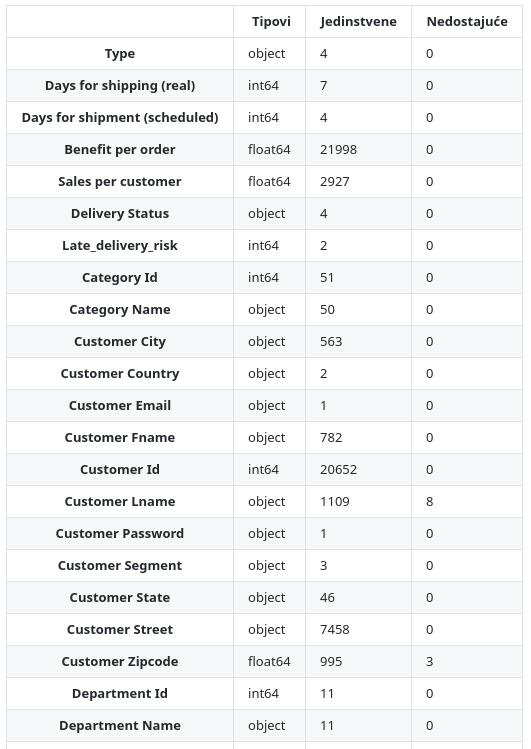
\includegraphics[width=8cm]{images/i12_Python-Anal-Table.png}
\centering
\caption{Analiza podataka}
\end{figure}

\chapter{Transakcijski Model Podataka}
\label{Ctrans}
Kako bi mogli napuniti skladište podataka prvo moramo stvoriti transakcijski model gdje se pohranjuju rezultati poslovnih procesa poput prodaja proizvoda, isporuka robe, itd. Nije opisano kako izgleda transakcijska baza podataka za preuzete podatke stoga sam stvorio svoju shemu. Odlučio sam iskoristiti što više atributa kako bih što vjerodostojnije izveo projekt.


\section{ER Dijagram}
ER dijagram prikazuje konceptualni model baze podataka. Neki skupovi atributa koji opisuju isti entitet su rastavljeni na dva entiteta.

\begin{figure}[h]
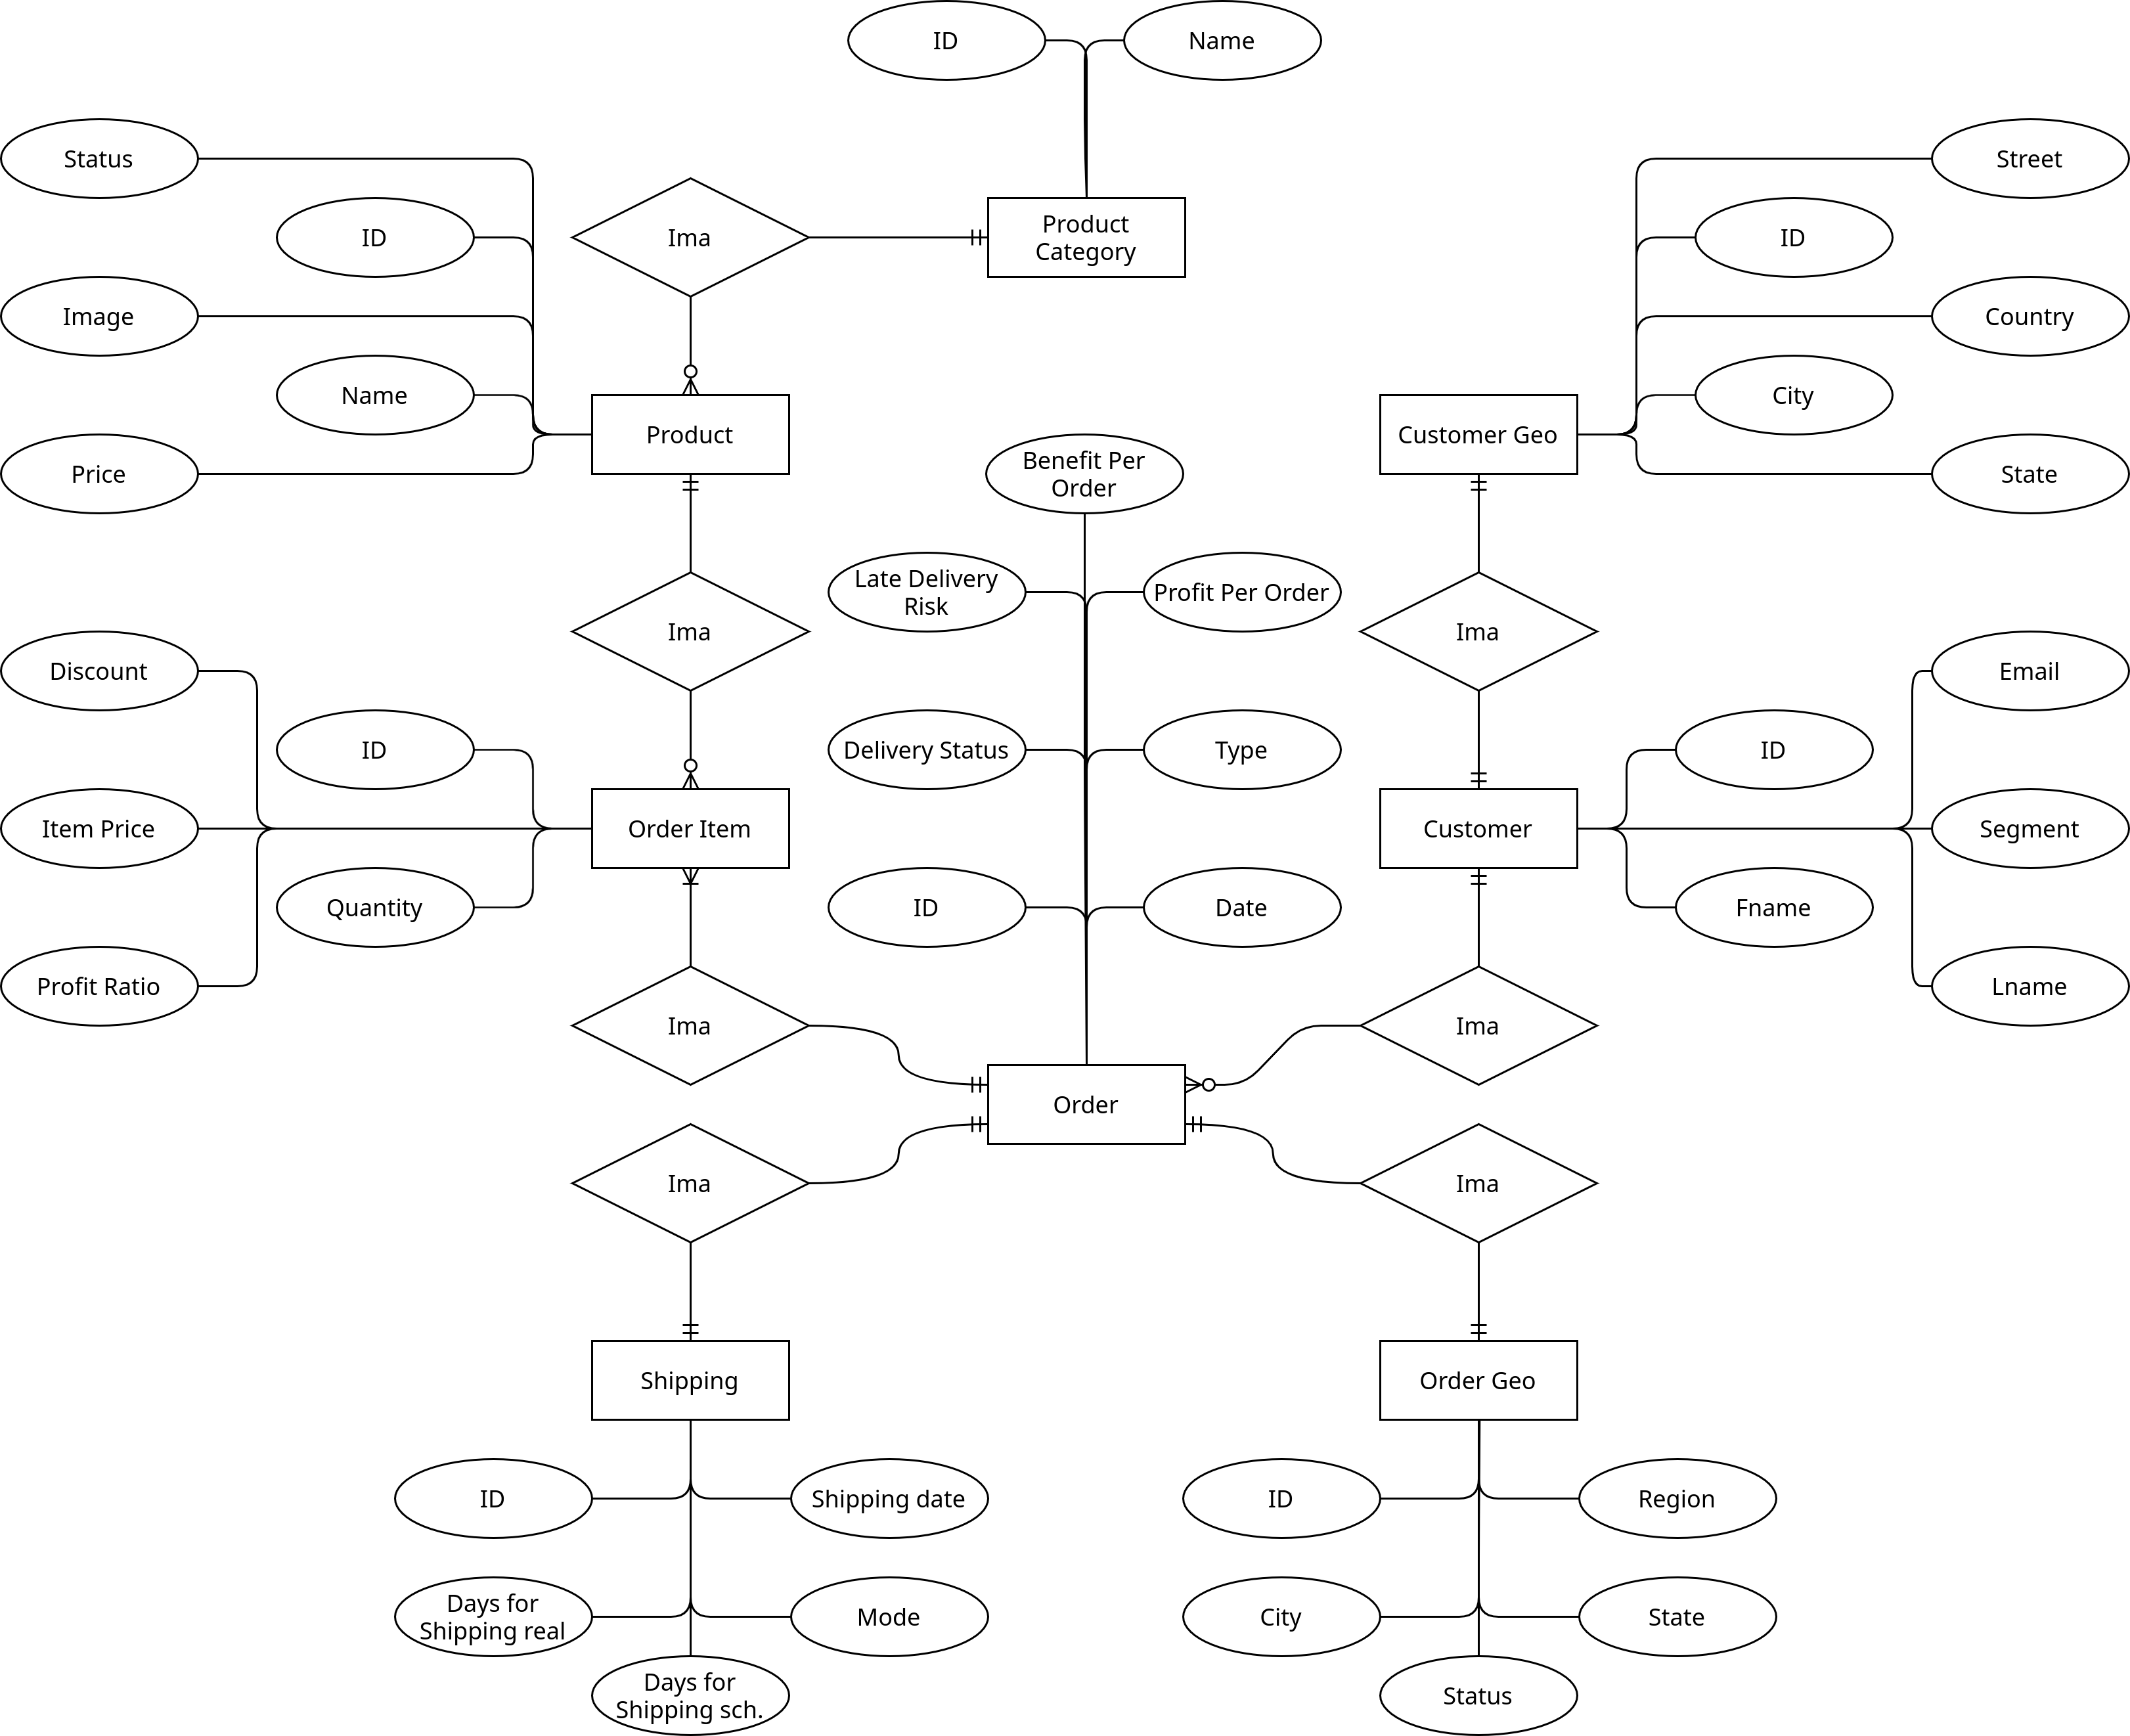
\includegraphics[width=16cm]{images/ER_Dijagram.png}
\centering
\caption{ER dijagram}
\end{figure}

\section{ER Model}
ER model se sastoji od 9 tablica koje opisuju poslovanje tvrtke koja prodaje neke proizvode. Svaka narudžba ima više stavki, poslovnicu, tablicu koja opisuje dostavu, kupca i njegovu geografsku lokaciju te svaka stavka sadrži opise o cijeni, količini, ukupnoj cijeni itd. 


\begin{figure}[h]
\includegraphics[width=16cm]{images/i01_data_co_schema.png}
\centering
\caption{ER model}
\end{figure}

\vspace{5cm}

\section{Punjenje Baze Podataka}



\subsection{CSV i SQL}
ER model se sastoji od ER model se sastoji od ER model se sastoji od ER model se sastoji od ER model se sastoji od ER model se sastoji od ER model se sastoji od ER model se sastoji od ER model se sastoji od ER model se sastoji od ER model se sastoji od 

\begin{figure}[h]
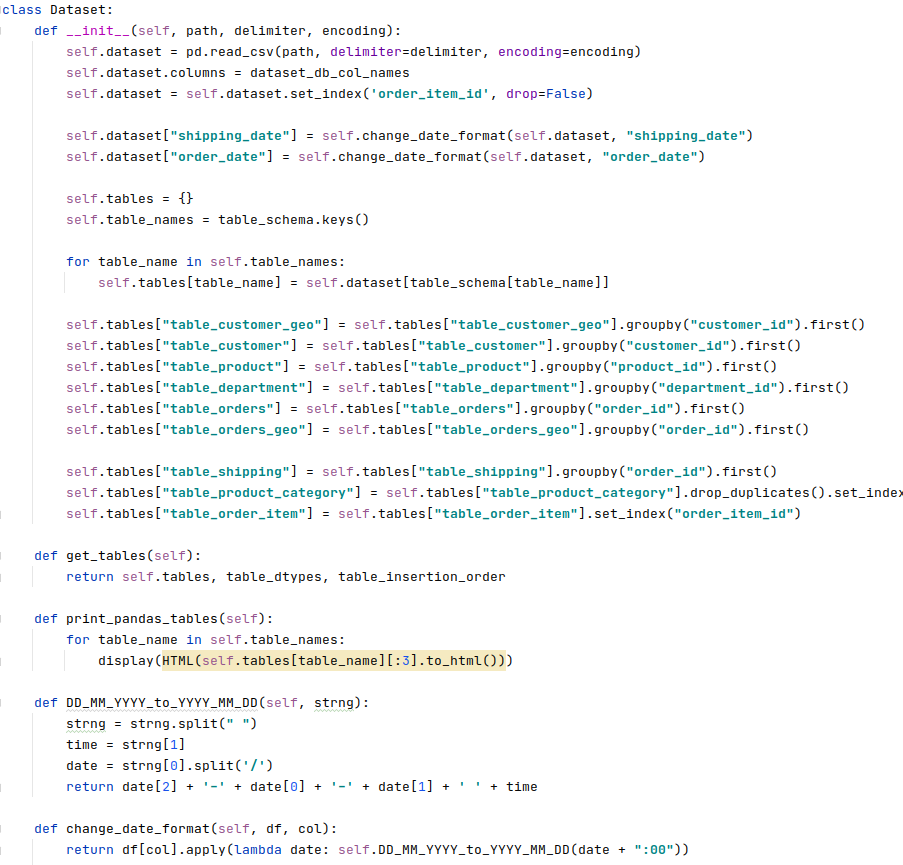
\includegraphics[width=14cm]{images/i15_Python-Table-Clean.png}
\centering
\caption{Python klasa za formatiranje podataka iz CSV datoteke}
\end{figure}



\begin{figure}[h]
\includegraphics[width=15cm]{images/i16_Python-Table-Desc.png}
\centering
\caption{Opisi tablica u Pythonu}
\end{figure}



\subsection{Python}


Transakcijski model podataka se puni uz pomoću Python skripte koja osim punjenja tablica također stvara novog korisnika i sheme za transakcijski i dimenzijski model. Za spajanje s bazom iz Python-a je korištena biblioteka SqlAlchemy a za formatiranje podataka Pandas. Potrebno je bilo samo formatirati datum jer su ostali podaci bili dovoljno dobri za korištenje.

\begin{figure}[H]
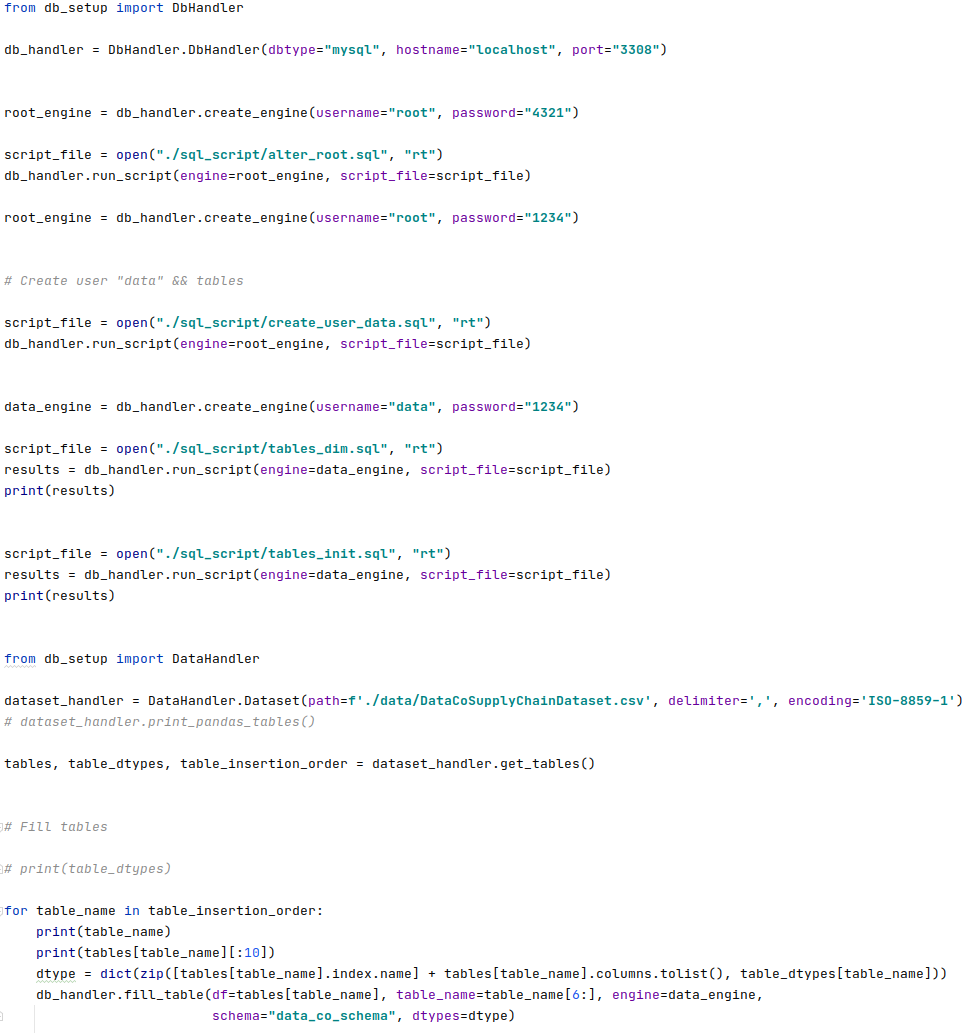
\includegraphics[width=15cm]{images/i14_Python-Init.png}
\centering
\caption{Python kod za inicijalizaciju baze podataka}
\end{figure}

Kako bih si olakšao punjenje baze stvorio sam dvije Python klase, jedna mi služi za stvaranje objekta koji ostvaruje vezu s bazom i izvršava SQL skripte dok druga klasa ima definirane SqlAlchemy tipove podataka, učitava CSV datoteku, izvršava čišćenje podataka i formatiranje podataka za transakcijski model. 


\subsection{Docker}
Docker Compose datoteka sadrži opis tri containera koja se nalaze na istoj virtualnoj mreži kako bi mogli međusobno komunicirati preko IP adrese i sadrže portove koji su vidljivi računalu. Koristio sam Docker jer mi je bilo puno lakše testirati ispravnost koda, nisam morao brisati sheme i sl. nego bi samo pokrenuo containere i Pyhthon skriptu te bih time dobio novu "čistu" bazu na kojoj mogu testirati ETL procese.

\begin{figure}[h]
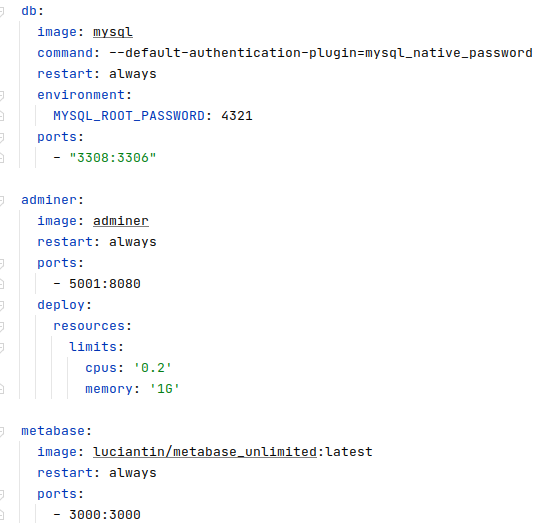
\includegraphics[width=12cm]{images/i01_Dockerfile.png}
\centering
\caption{Docker Compose definicije containera}
\end{figure}

\chapter{Dimenzijski Model Podataka}
\label{Cdim}
Kako bi mogli pratiti promijene podataka, svaka tablica sadrži atribute "date\_from" i "date\_to" pomoću kojih možemo odrediti od kada i do kada je neki zapis aktivan. Modelirano je tako da dimenzijski model podržava promijene narudžba i stavki narudžba osim samo njihovih dimenzija jer je prodaja proizvoda dinamička, kupac se može predomisliti nakon što naruči proizvode te ovim modelom možemo pratiti te promijene i bolje razumjeti potrebe kupaca. Dimenzijski model se sastoji od četiri dimenzije, dvije tablice činjenica i jedne tablice koja služi za spajanje tablica činjenica. Svaka tablica sadrži primarni ključ kojim je svaki zapis povezan s izvorišnom bazom podataka te se time može lakše ažurirati stanje.

\begin{figure}[h]
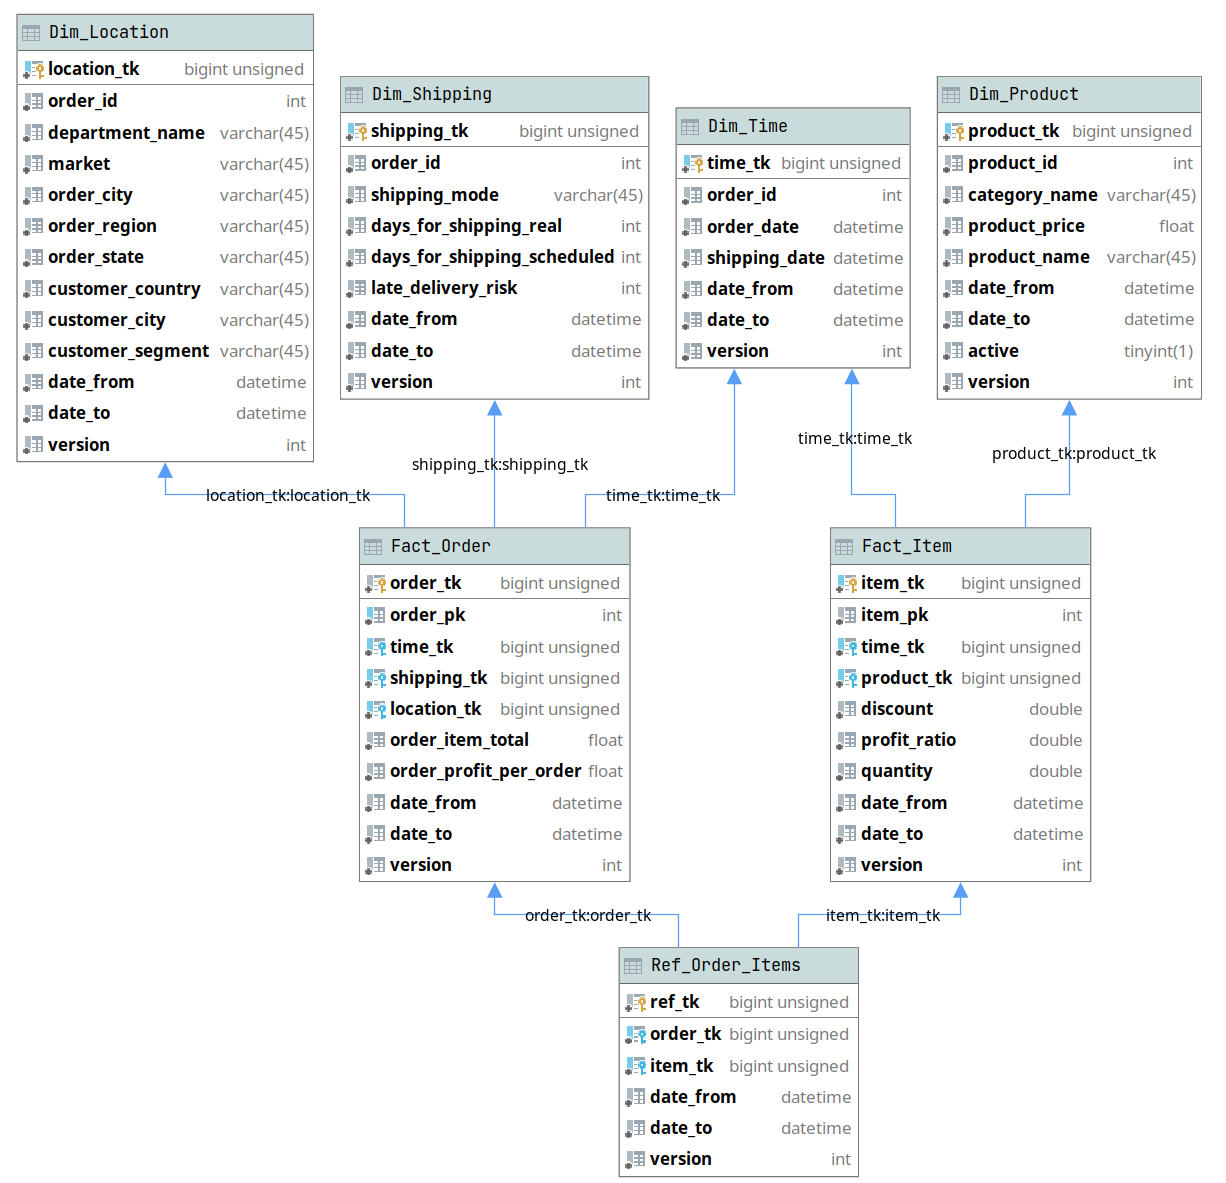
\includegraphics[width=10cm]{images/i02_data_co_schema_dim.png}
\centering
\caption{Dijagram servisa}
\end{figure}

Dimenzija "Location" opisuje adresu dostave, adresu kupca, tip tržišta kupca (dali je to privatni korisnik, tvrtka, itd.) te poslovnicu koja je obradila tu narudžbu. Dimenzija "Time" sadrži dva datuma, kada je korisnik naručio proizvode i kada je proizvod isporučen. Dimenzija "Product" opisuje tip proizvoda te je povezana s tablicom činjenica "Fact\_Item" i služi za opis tog proizvoda. Dimenzija "Shipping" opisuje koliko je dana bilo potrebno za isporuku proizvoda i sadrži način dostave. Tablica činjenica "Fact\_Order" opisuje narudžbe, profit i ukupnu vrijednost proizvoda, dok tablica činjenica "Fact\_Item" opisuje pojedinu stavku narudžbe. Stavka narudžbe ima atribute koji opisuju popust, ostvareni profit i količinu proizvoda. Za postavljanje baze podataka koristim tri SQL datoteke sa DDL i DCL naredbama, dvije sadrže naredbe za izradu sheme dok jedna SQL datoteka sadrži naredbe za stvaranje korisnika, izmjenu lozinke root korisnika i postavljanje pravila korisnika koji upravlja transakcijskom i dimenzijskom shemom.



\chapter{ETL Procesi}
\label{Cetl}
ETL procesi služe za ekstrakciju, transformaciju i punjenje dimenzijskog modela, sve dimenziju su sporo mijenjajući dimenzije tipa 2, sadrže verziju dimenzijskog unosa u atributu "version" i datume koji opisuju interval u kojem je zapis aktivan . Ažuriranje dimenzijskog modela se izvršava pomoću elementa "Dimension lookup/update" koji se brine o unosu datuma, verzije i tehničkog ključa \cite{pentaho}. Svaka tablica dimenzijskog modela sadrži primarni ključ kojim je zapis povezan s zapisom u transakcijskoj bazi te se time lakše ažuriraju vrijednosti.

\section{Pentaho "Job"}
Sve ETL transformacije se izvršavaju u dva Pentaho Job-a. Sveukupno se koriste 6 transformacija za punjenje dimenzijskog modela, 4 transformacije za punjenje dimenzijskih tablica, jedna transformacija za punjenje obje tablice činjenica i jedna transformacija za punjenje tablice kojom se spajaju tablice činjenica.


Dimenzije se pune paralelno jer ne ovise jedna o drugoj, slika \ref{UpdateDim} . Nakon što se taj Pentaho job izvrši onda se krene na sljedeće transformacije u glavnom jobu, prikazan slikom 5.2 .

\begin{figure}[H]
\label{PentahoUpdateA}
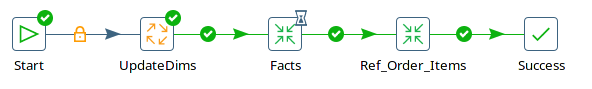
\includegraphics[width=16cm]{images/i10_Pentaho-Update-Facts.png}
\centering
\caption{Glavni Pentaho "Job"}
\end{figure}

\begin{figure}[H]
\label{UpdateDim}
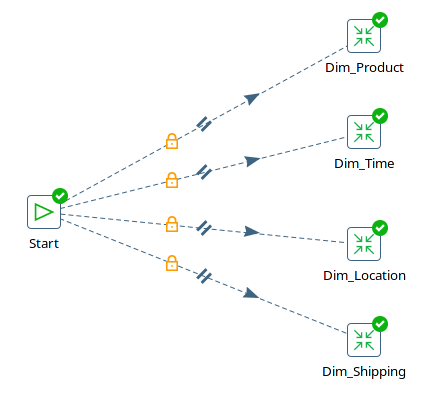
\includegraphics[width=16cm]{images/i09_Pentaho-Update-Dim.png}
\centering
\caption{Punjenje dimenzija}
\end{figure}

\vspace{8cm}

\section{Transformacije}


\subsection{Dimenzija Vrijeme}
Vremenska dimenzija sadrži dva atributa koji opisuju vrijeme kada je narudžba donesena i kada je dostavljena. Atributi se nalaze u različitima tablicama pa se moraju prvo tablice spojiti prije punjenja dimenzije.

\begin{figure}[H]
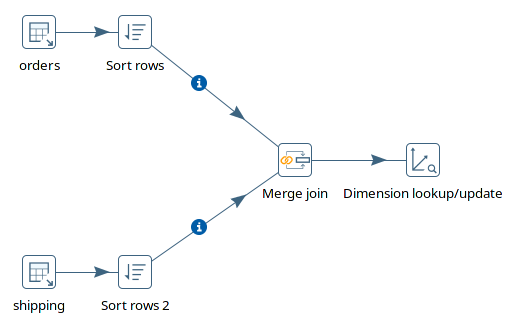
\includegraphics[width=16cm]{images/i05_Pentaho-Dim-Time.png}
\centering
\caption{Punjenje vremenske dimenzije}
\end{figure}
\subsection{Dimenzija Dostava}
Sadrži atribute koji opisuju dostavu pojedine narudžbe, način dostave, dani potrebni za dostavu te rizik za zakašnjenje dostave. Puni se uz pomoć podataka iz tablice "Shipping" i CSV datoteke, ti podaci se tada sortiraju, spoje i selektiraju se samo potrebni atributu. Dimenzija se puni samo s jedinstvenim vrijednostima zato što je CSV datoteka denormalizirana te se, po primarnom ključu narudžba, moraju maknuti duplikati koji su nastali zbog toga što svaka narudžba ima više stavki. 
\begin{figure}[H]
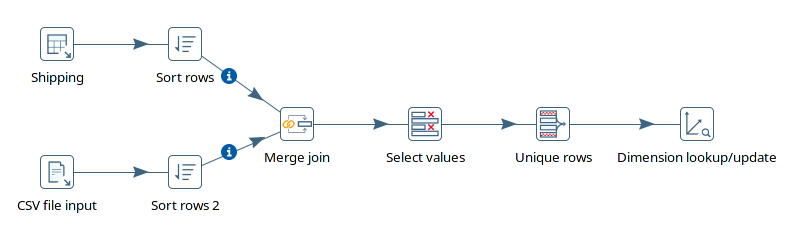
\includegraphics[width=16cm]{images/i04_Pentaho-Dim-Shipping.png}
\centering
\caption{Punjenje dimenzije dostava}
\end{figure}

\vspace{3cm}

\subsection{Dimenzija Proizvod}
Dimenzija proizvod opisuje proizvod u tablici činjenica za stavke narudžba. Sadrži naziv proizvoda, cijenu i naziv kategorije koj taj proizvod pripada. Osim što spajanja podataka iz CSV datoteke i tablice, dodao sam i atribut koji označuje jeli proizvod trenutno aktivan ali nije bilo potrebno jer se isto može postići s datumima koji se unose u "Dimension lookup/update" elementu. 

\begin{figure}[H]
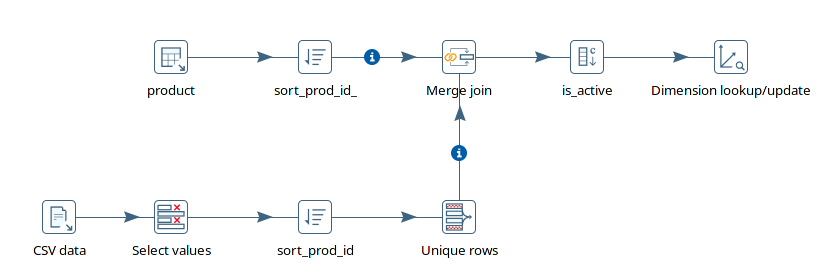
\includegraphics[width=16cm]{images/i03_Pentaho-Dim-Product.png}
\centering
\caption{Punjenje dimenzije proizvod}
\end{figure}
\subsection{Dimenzija Lokacija}
Slika \ref{DimLoc} prikazuje Pentaho transformaciju koja prikuplja lokacije iz više tablica te ih spaja s primarnim ključem narudžba. Podaci se sortiraju ovisno o ključu pomoću kojeg se spajaju jer se spajaju pomoću različitih primarnih ključeva. Prije punjenja, odaberu se vrijednosti kojima će se napuniti dimenzija te se nakon toga dimenzija napuni zajedno s tehničkim ključem, datumima i verzijom.
 
\begin{figure}[H]
\label{DimLoc}
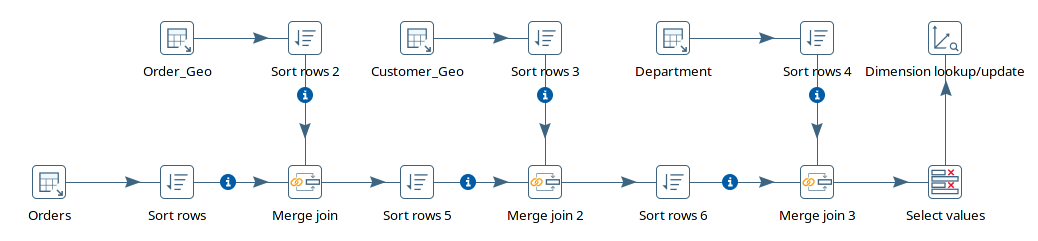
\includegraphics[width=16cm]{images/i02_Pentaho-Dim-Location.png}
\centering
\caption{Punjenje dimenzije lokacija}
\end{figure}

\vspace{5cm}

\subsection{Tablice Činjenica}
Kao što je ranije navedeno, koriste se dvije tablice činjenica, jedna prati ukupan profit i ukupnu cijenu za svaku narudžbu dok druga tablica činjenica prati količinu, , cijenu i popust stavke narudžbe. Obje sadrže atribute za praćenje od kad i do kada je aktivan pojedini zapis jer se pomoću toga mogu pratiti interesi kupaca, dali su odlučili nakon narudžbe zamijeniti neku stavku. Tablice činjenica sadrže primarni ključ kojim se stvara veza na transakcijski zapis iz kojega je preuzeta pojedina činjenica. Tablice činjenica se pune u istoj transformaciji jer je potrebno manje vremena zbog kopiranja sortiranih podataka dimenzijske tablice vremena. Umjesto da se dvaput sortira 160,000+ zapisa, oni se sortiraju jedanput, kopiraju i vežu s obje tablice činjenica.  



\begin{figure}[H]
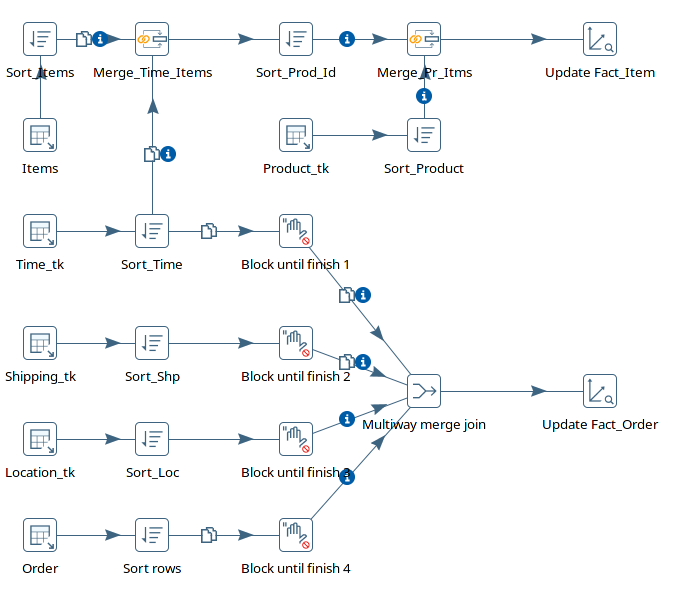
\includegraphics[width=16cm]{images/i06_Pentaho-Facts.png}
\centering
\caption{Dijagram servisa}
\end{figure}

\vspace{10cm}

\subsection{Spajanje Tablica Činjenica}
Kako bi se mogle tablice činjenica povezati, stvorena je tablica koja služi za povezivanje svakog tehničkog ključa tablice činjenica narudžba sa tehničkim ključevima tablice stavki. Tablica je usklađena dimenzija kojom se može iz jedne tablice činjenica doći do druge, no ona ne sadrži nikakve atribute koji opisuju tu vezu. Kao i ostale tablice dimenzijskog modela, i ova tablica je napravljena tako da prati povijesne podatke. Slika \ref{RefOrder} prikazuje izgled tog ETL procesa, prvo se dohvate originalni podaci iz transakcijske baze kako bi se mogli spojiti točni tehnički ključevi. Zatim se dohvaćeni primarni ključevi narudžba i stavki spajaju s posebno dohvaćenom tablicom činjenica stavki narudžbe te se nakon toga spajaju s tablicom činjenica za narudžbe i onda se dimenzijski model ažurira.  

\begin{figure}[H]
\label{RefOrder}
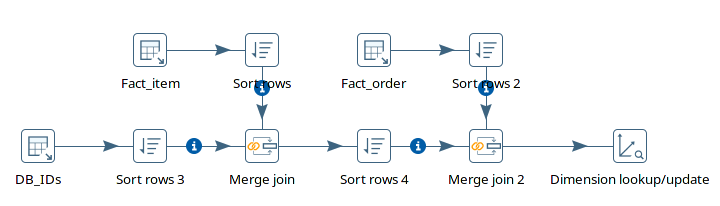
\includegraphics[width=16cm]{images/i07_Pentaho-Ref-Order-Items.png}
\centering
\caption{Dijagram servisa}
\end{figure}

\chapter{Vizualizacija Podataka}
\label{Cviz}
Podaci se vizualiziraju kako bi pomogli u odlučivanju, stoga sam odlučio vizualizirati par različitih upita koji mislim da su važni za donošenje odluka o poslovanju tvrtke. Za vizualizaciju je korišten Metabase jer je otvoren kod, te je to web aplikacija koja se može lokalno pokrenuti uz pomoć Docker-a.

\section{Metabase}
Kako bih mogao koristiti Metabase sa velikom količinom podataka, morao sam zamijeniti par vrijednosti koje određuju gornju granicu dohvaćanja zapisa. Stvorio sam svoju Metabase sliku i postavio sam ju na DokcerHub. Metabase se sastoji od više elemenata, nadzorna ploča služi za prikazivanje više grafova dok su grafovi stvoreni uz pomoć posebnog alata koji omogućuje lakše postavljanje upita i odabira tipa grafa.

\subsection{Dizajn Upita}
Upiti se stvaraju tako da se odabere početna tablica nakon čega se podaci mogu spojiti s drugim tablicama, može se stvoriti novi atribut od dobijenih atributa te se još podaci mogu grupirati, filtrirati ili se može ograničiti broj dohvaćenih zapisa.  Slika \ref{UpitiDizajn} prikazuje upit kojim se dohvaćaju podaci o ukupnoj prodaji svakog proizvoda.


\begin{figure}[H]
\label{UpitiDizajn}
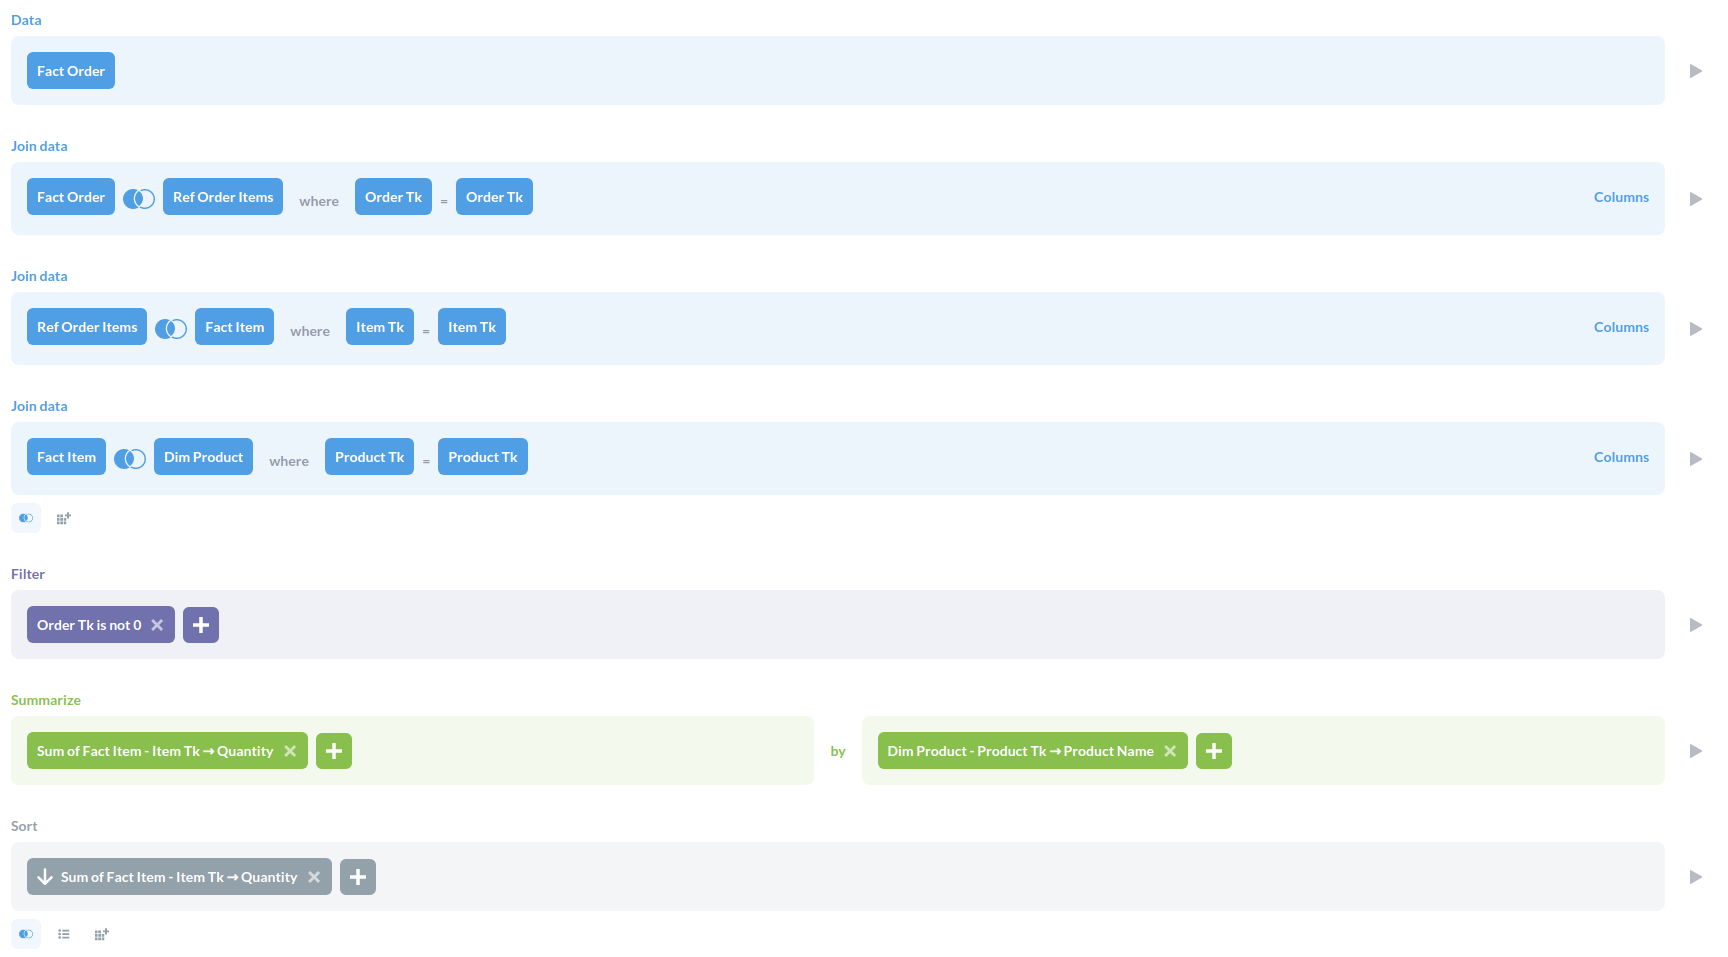
\includegraphics[width=16cm]{images/Metabase-TotalItemsSold-Editor.png}
\centering
\caption{Upit kojim se dohvaćaju podaci o ukupnoj prodaji proizvoda}
\end{figure}


\subsection{Nadzorna ploča}
Nakon što se graf spremi, on se može dodati na neki od nadzornih ploča gdje mu se može promijeniti veličina, boja, pozicija te se određenim tipovima grafova može dodati više serija podataka, kako bi se prikazalo više grafova u jednom.


\begin{figure}[H]
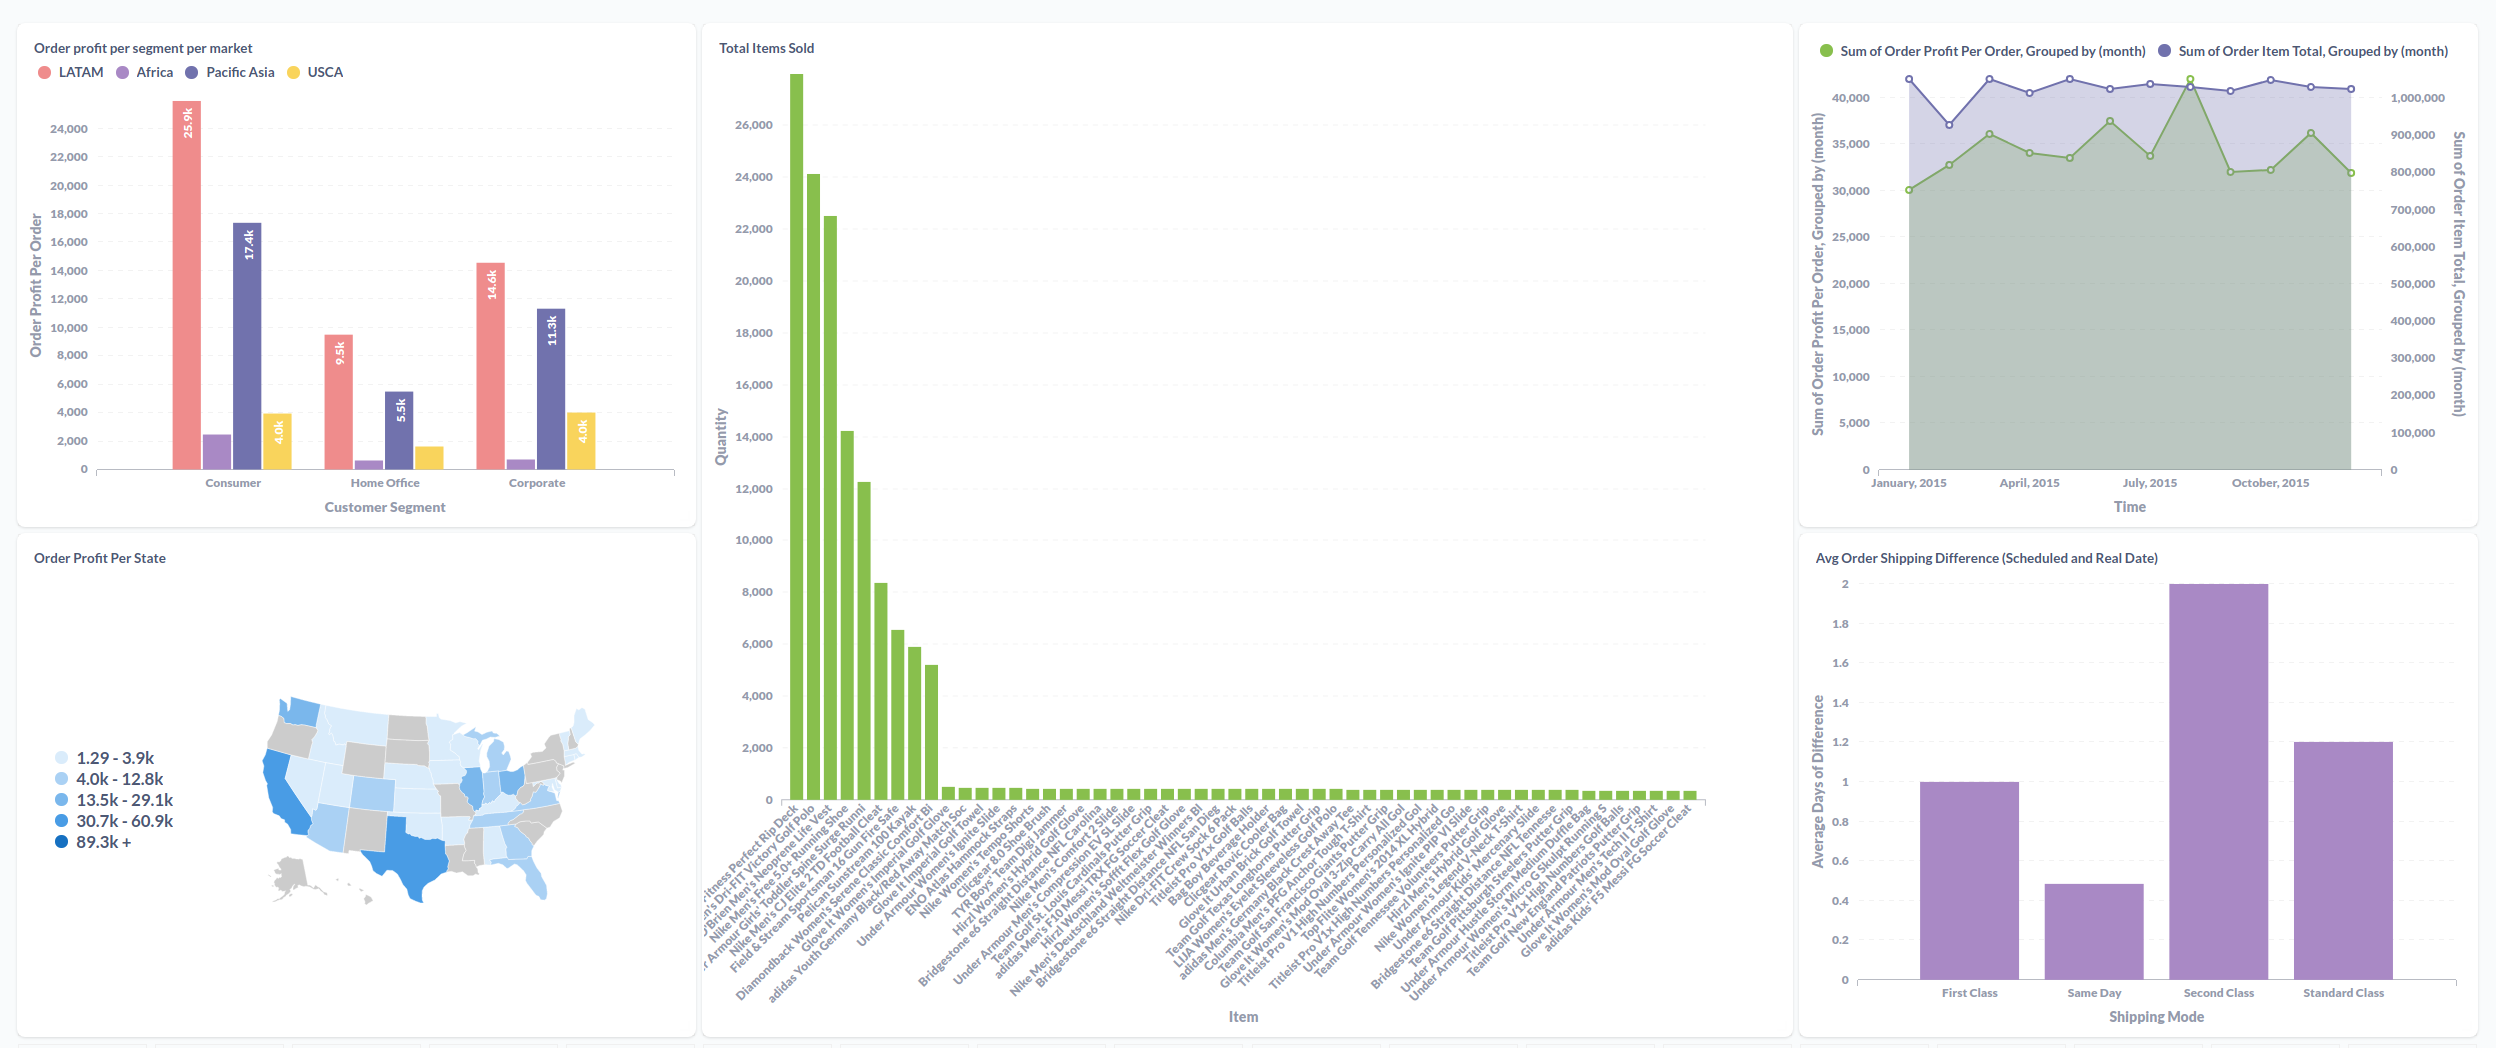
\includegraphics[width=16cm]{images/Metabase-Dasboard.png}
\centering
\caption{Dijagram servisa}
\end{figure}


\section{Vizualizacije}
Cilj vizualizacija podataka je zadovoljiti potrebe menadžera stoga sam odabrao  prikazati na geografskoj karti frekvenciju narudžba u pojedinim državama SAD-a, prikazati koji se proizvodi najčešće naručuju, profit narudžba ovisno o segmentu kupaca u svakom tržištu, ukupnu cijenu narudžbe i ostvarenoga profita u nekom vremenskom intervalu i prosječnu razliku između stvarnih dana potrebnih za dostavu i zakazanih dana, grupirano po tipu dostave. 



\subsection{Ukupna cijena narudžbe i profit u vremenskom intervalu}
Slika \ref{OrderTotalProfit} prikazuje ukupnu cijenu narudžbe ljubičastom bojom te je na tu vremensku seriju dodan drugi graf koji prikazuje ukupan profit. Vremensko razdoblje je jedna godina te su podaci sumirani za svaki mjesec u toj godini.

\begin{figure}[H]
\label{OrderTotalProfit}
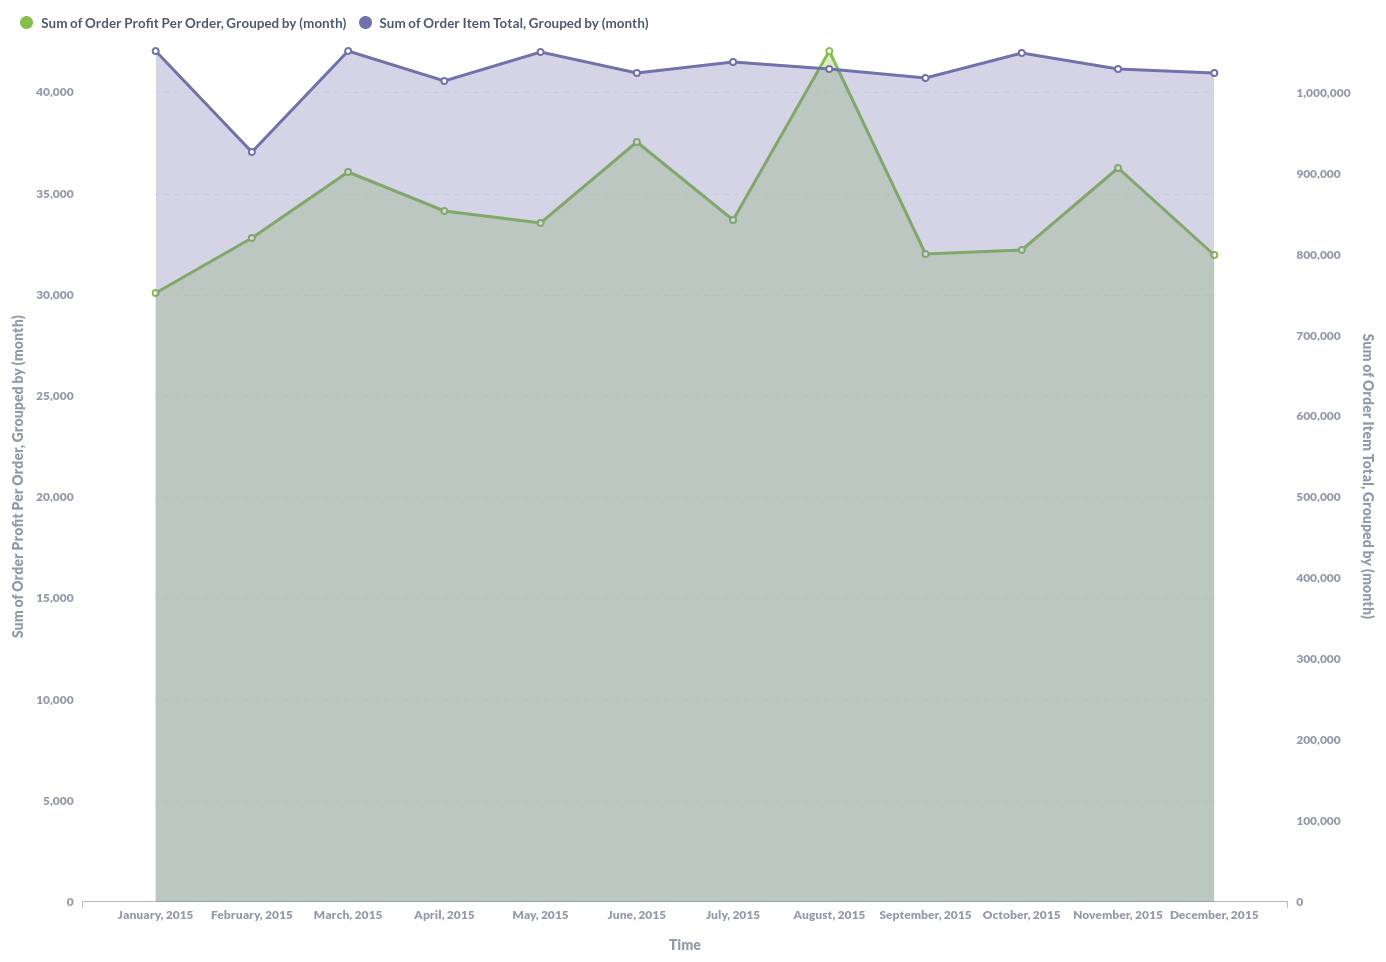
\includegraphics[width=16cm]{images/Metabase-OrderTotalProfit.png}
\centering
\caption{Dijagram servisa}
\end{figure}

\subsection{Dobit od narudžbe po tržištu, po segmentu kupaca}

Slika \ref{ProfitSegment} prikazuje ostvarenu dobit po tržištu, te su podaci, unutar svakog tržišta, grupirani po segmentu kupaca.

\begin{figure}[H]
\label{ProfitSegment}
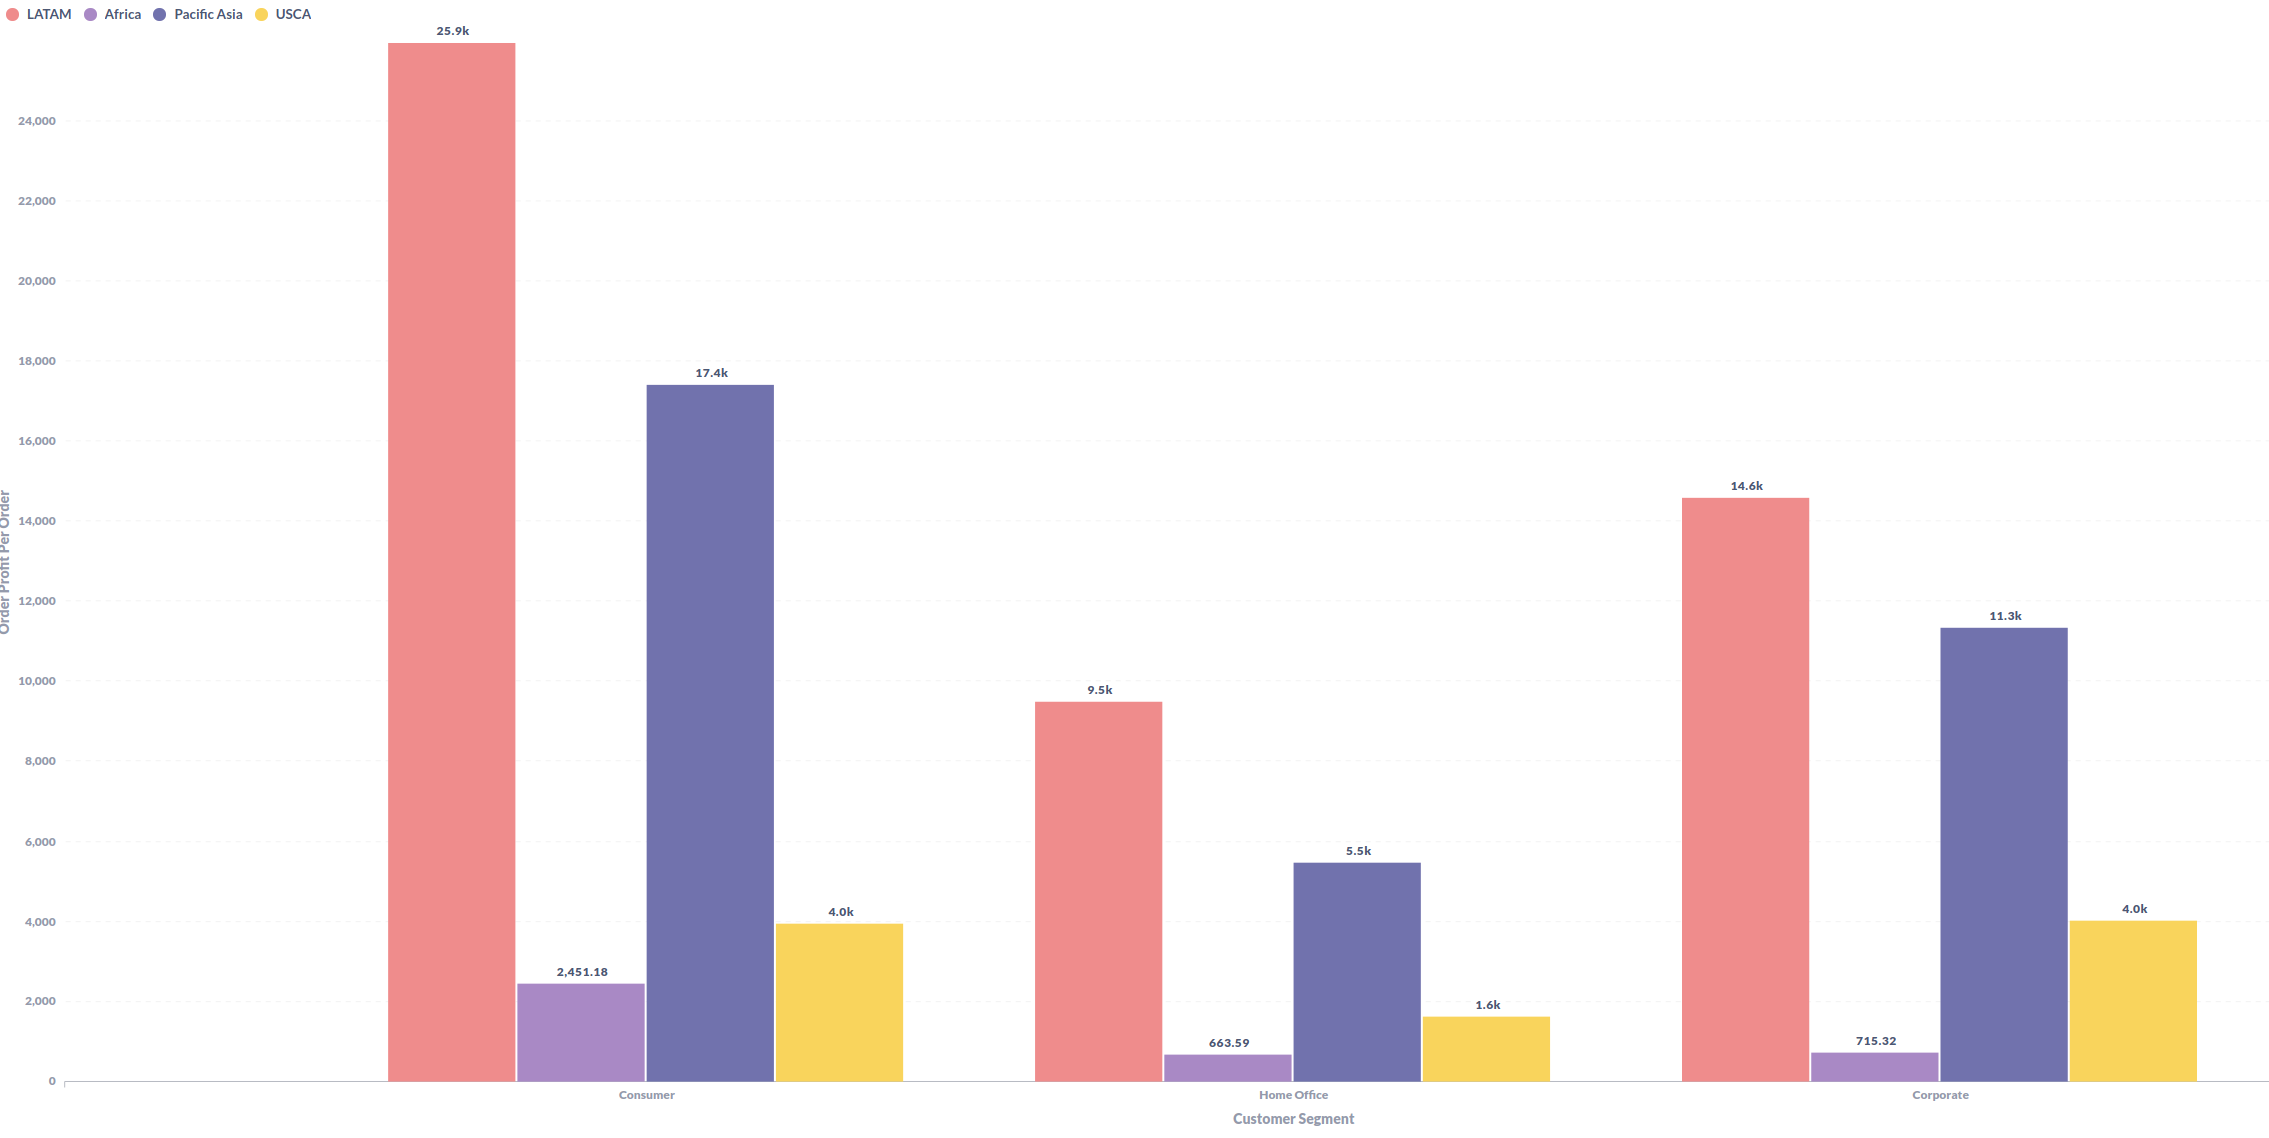
\includegraphics[width=16cm]{images/Metabase-ProfitSegment.png}
\centering
\caption{Dijagram servisa}
\end{figure}


\subsection{Prosječna razlika u zakazanim danima dostave i stvarnim danima dostave po načinu dostave}
Graf na slici \ref{ShippingDiff}, za svaki tip dostave, prikazuje prosječnu razliku između zakazanih dana potrebnih za dostavu i stvarnih dana koliko je trebalo da se narudžba dostavi. Ovime se može vidjeti dali tvrtke, uz pomoć kojih se dostavljaju proizvodi, pružaju dovoljno dobru uslugu našim kupcima.   

\begin{figure}[H]
\label{ShippingDiff}
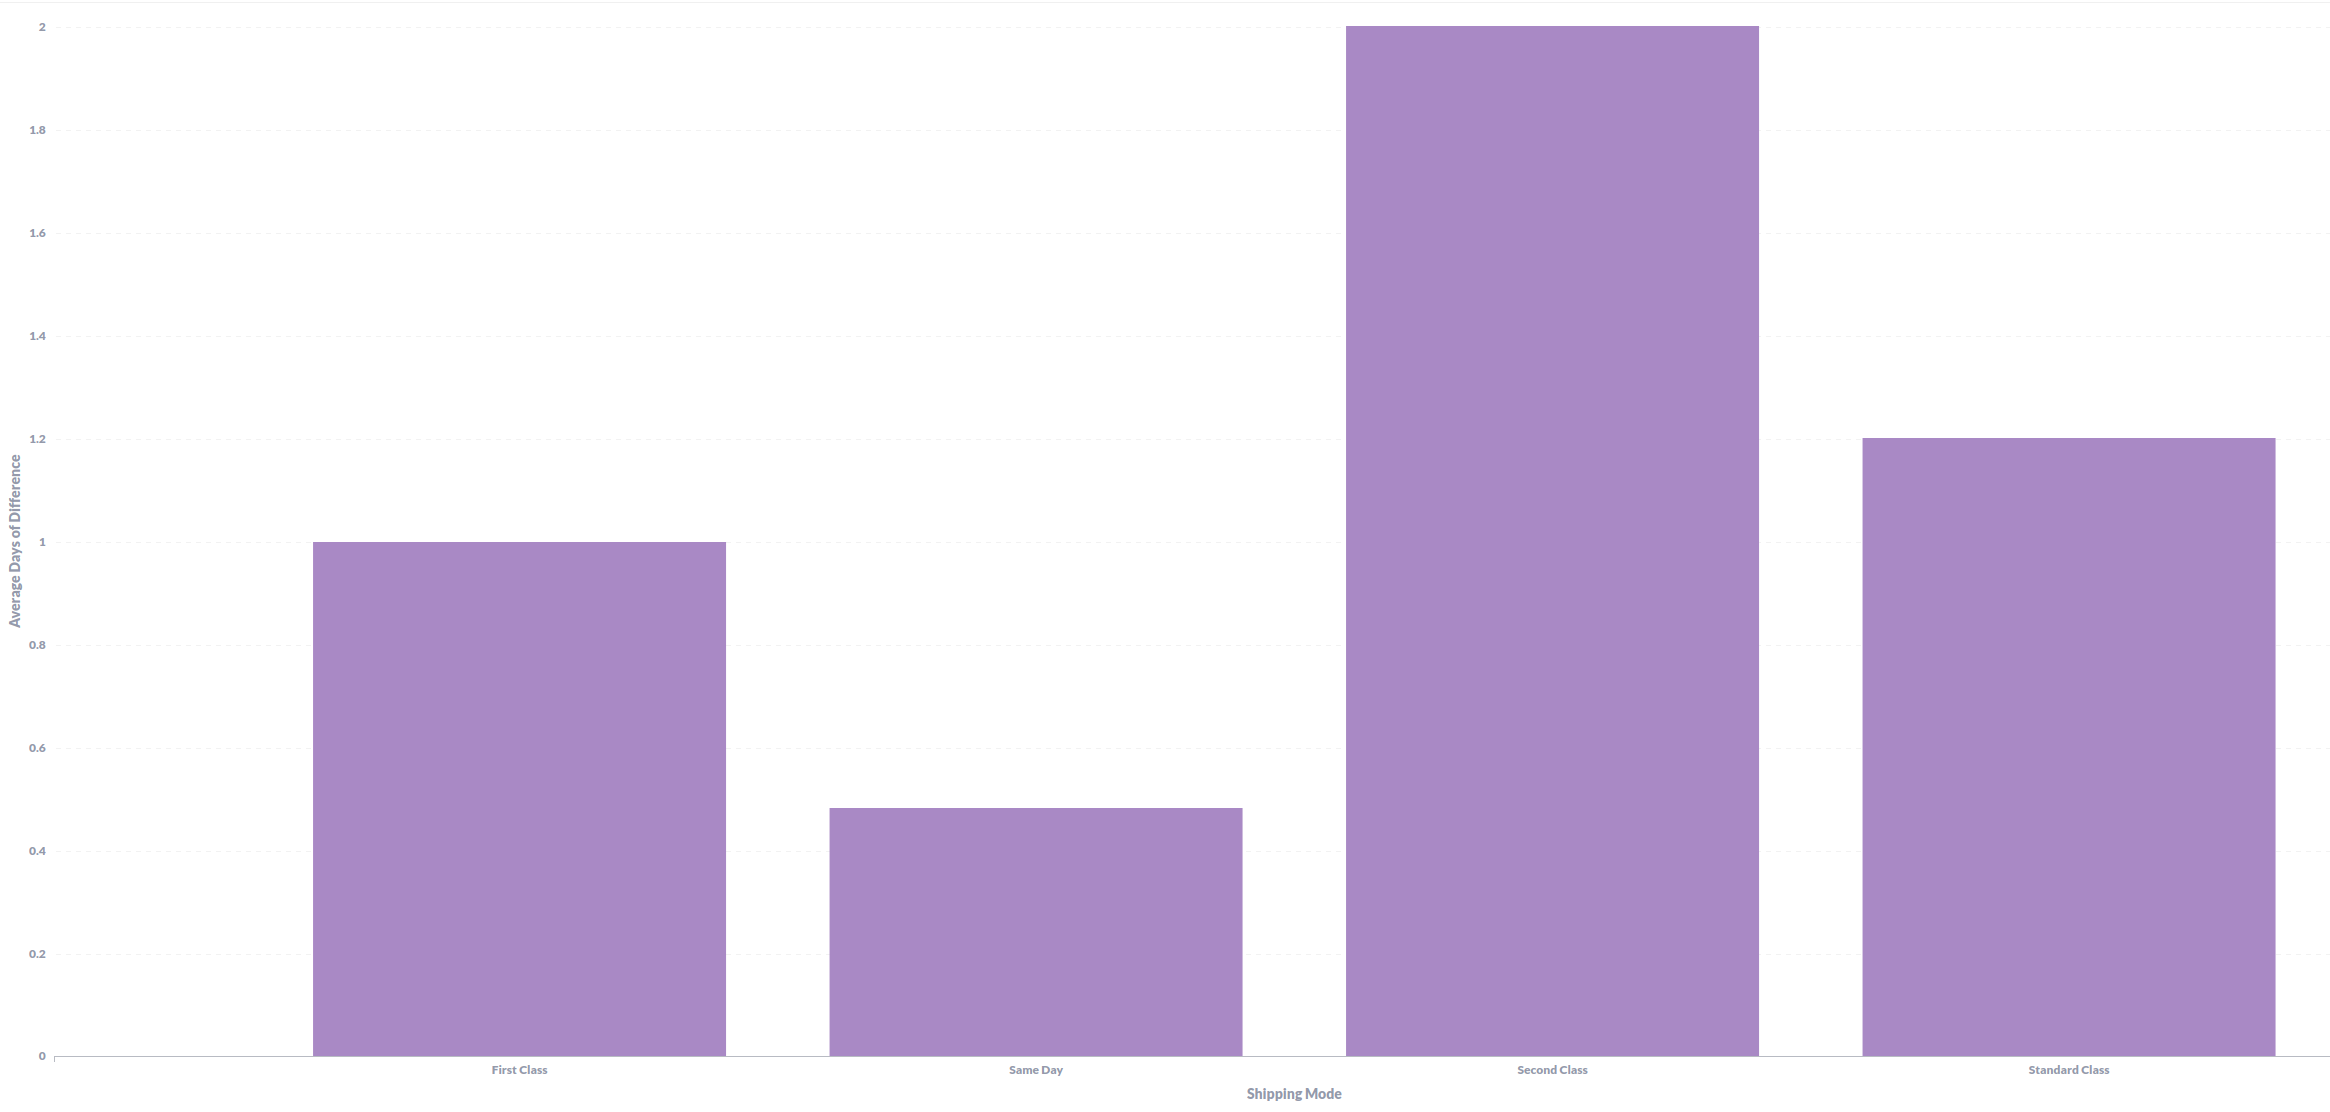
\includegraphics[width=16cm]{images/Metabase-ShippingDiff.png}
\centering
\caption{Dijagram servisa}
\end{figure}


\subsection{Dobit po narudžbi po državi}
Kako bismo vidjeli u kojim državama najbolje poslujemo a u kojima najlošije, na karti SAD-a sam prikazao sumu profita za svaku državu. 

\begin{figure}[H]
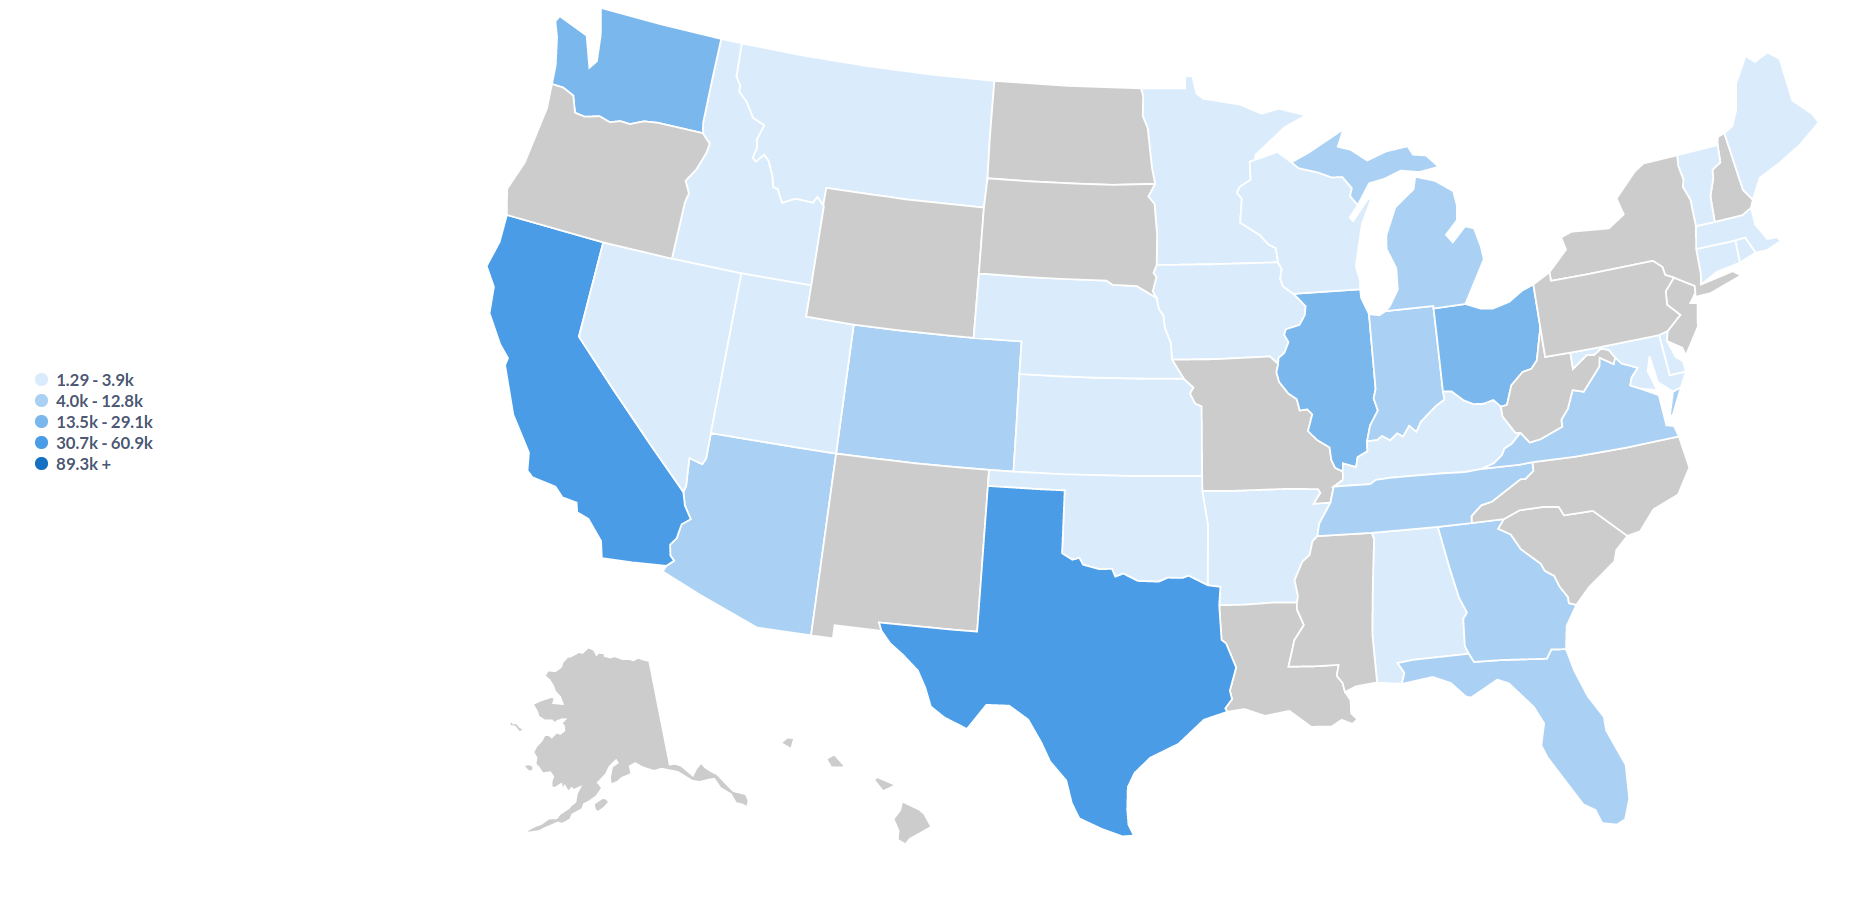
\includegraphics[width=16cm]{images/Metabase-State.png}
\centering
\caption{Dijagram servisa}
\end{figure}

\subsection{Ukupna količina prodanih proizvoda}
Kako bi se moglo vidjeti koji su proizvodi najuspješniji, vizualizirao sam ukupnu količinu prodanih proizvoda. 

\begin{figure}[H]
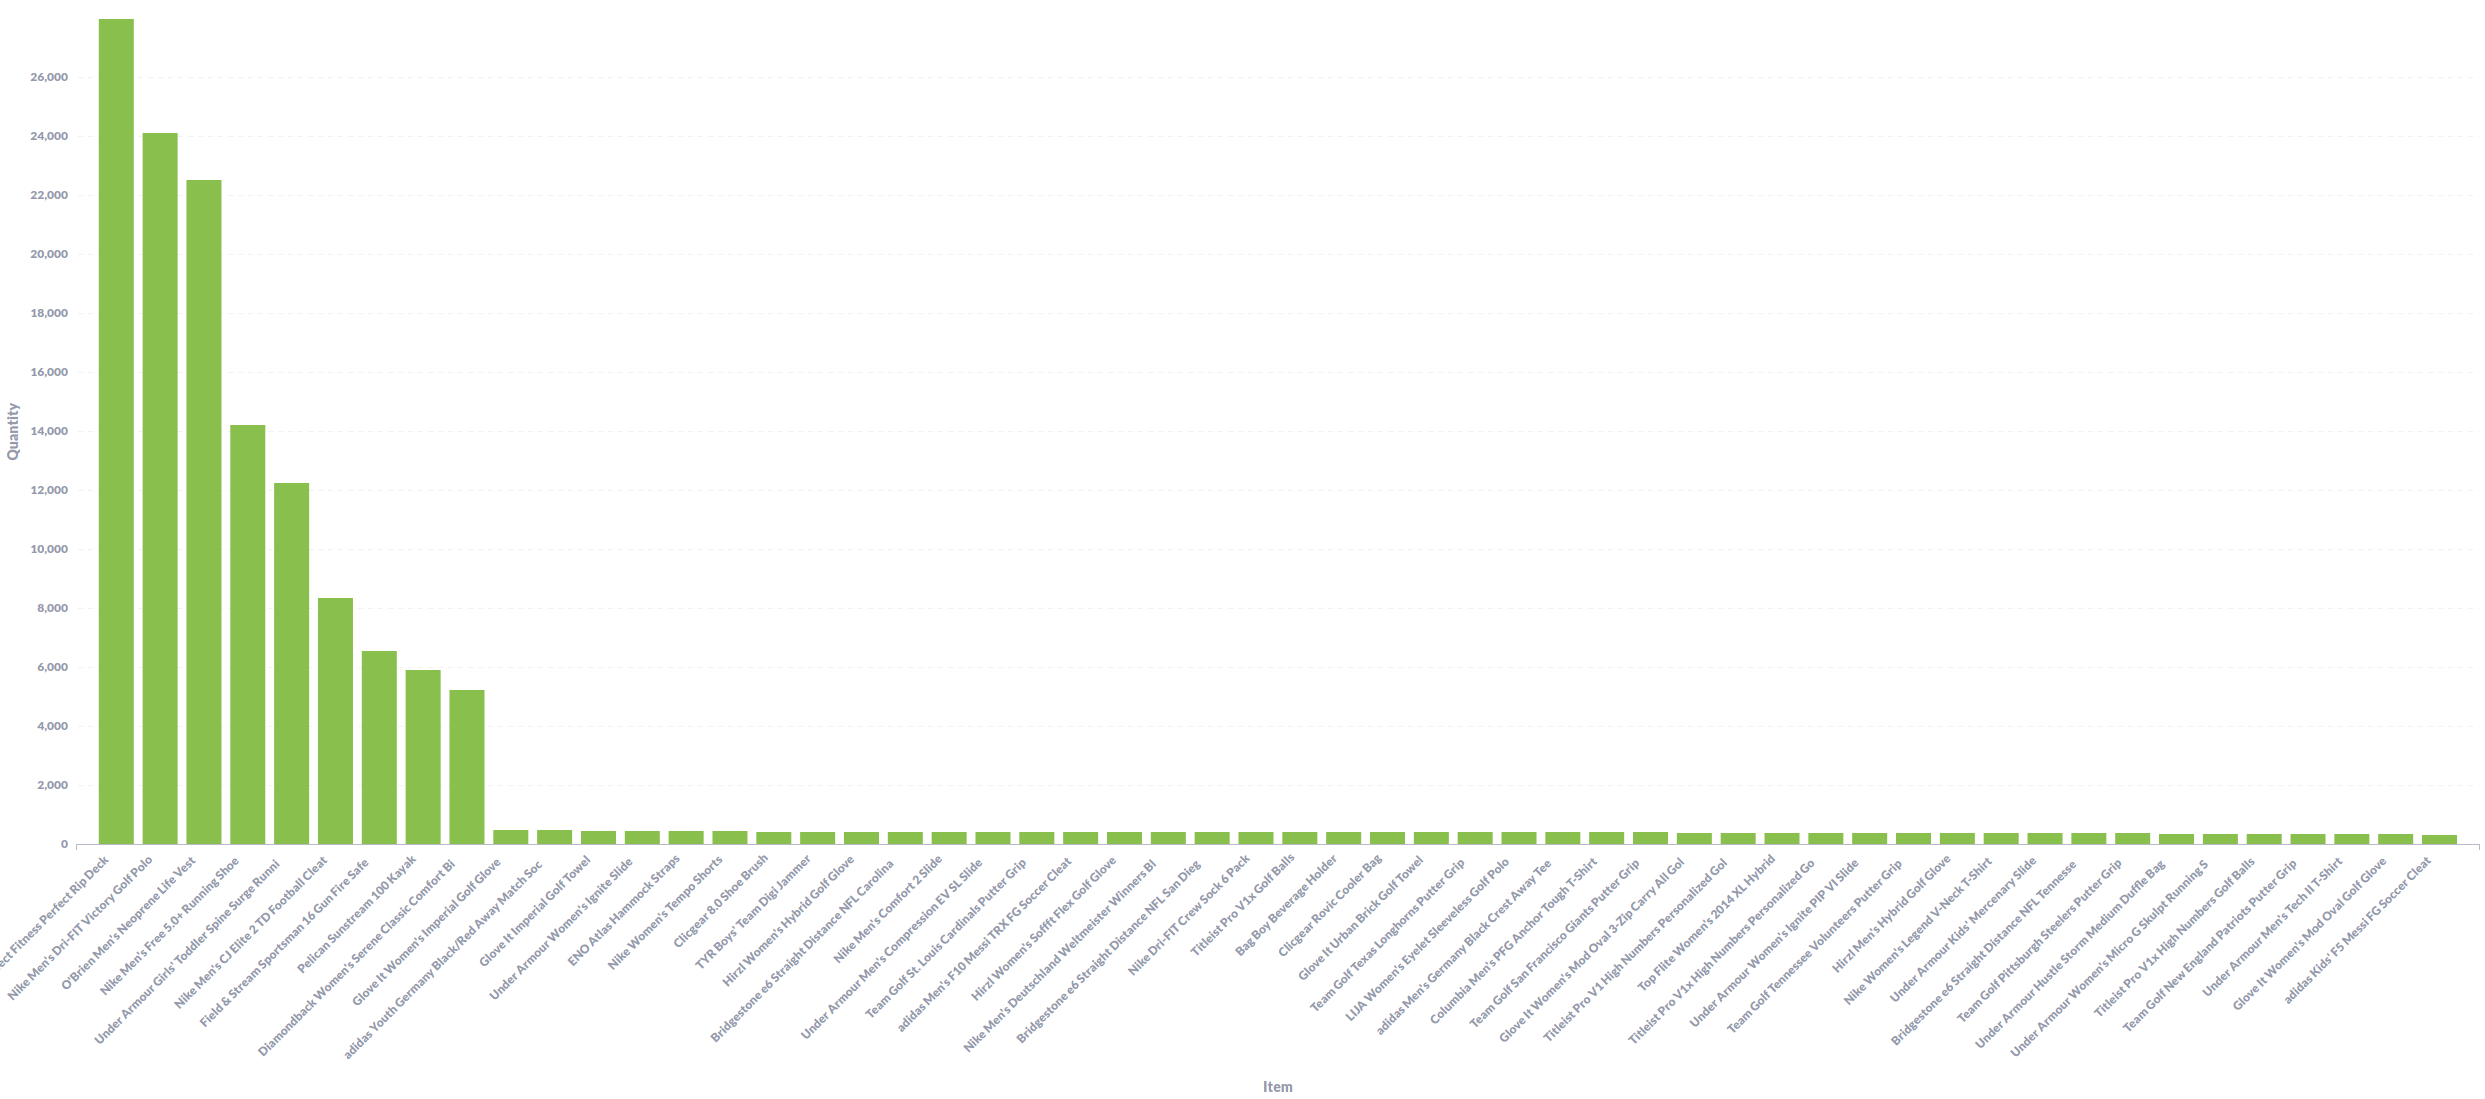
\includegraphics[width=16cm]{images/Metabase-TotalItemsSold.png}
\centering
\caption{Dijagram servisa}
\end{figure}



\chapter{Zakljucak}

Kroz ovaj rad prikazan je proces stvaranja skladišta podataka, punjenje i vizualizacija podataka. Projekt je izrađen uz pomoć raznih alata i programskih rješenja kako bi se dobila nadzorna ploču u kojoj su vidljivi podaci o poslovanju tvrtke. Denormalizirani podaci, koji opisuju rad tvrtke, pune se uz pomoć Python-a koji također transformira te podatke kako bi se mogli prenijeti u transakcijsku bazu podataka. ETL procesi su dizajnirani tako da se podaci mogu lagano ažurirati na novije stanje, te se za punjenje dimenzijskog modela koriste podaci iz različitih izvora. Program za vizualizaciju podatak je morao biti izmjenjen kako bi mogao prikazati velike količine podataka te je također korišten Docker kako bi se projekt mogao pokrenuti na raznim računalima bez utjecaja nečije okoline. 




\clearpage
\pagestyle{plain}

\renewcommand\bibname{{Reference}} 

\printbibliography


\end{document}
